\documentclass[12pt]{article}
\usepackage[utf8]{inputenc}
\usepackage{chemfig}
\usepackage[version=4]{mhchem}
\usepackage{amsfonts}
\usepackage{amsmath}
\usepackage{amssymb}
\usepackage{geometry}
\usepackage{mathabx}
\usepackage{relsize}
\usepackage{graphics}
\usepackage[colorlinks = true,
            linkcolor = blue,
            urlcolor  = blue,
            citecolor = blue,
            anchorcolor = blue]{hyperref}
%\usepackage{indentfirst}
\usepackage{tikz}
\usepackage{listings}
\usepackage{sidecap}
\usepackage{comment}
\geometry{
 a4paper,
 total={6.5in,0in},
 left= 15mm,
 top= 15mm,
 bottom=15mm,
 right = 15mm
 }
\title{Energy Log}
\author{Marcos Perez}
\date{June 2022 - }

\begin{document}

\maketitle

\section{June-ish}
\subsubsection{5/31/22}
Configuring \href{https://docs.github.com/en/repositories/working-with-files/managing-large-files/configuring-git-large-file-storage}{https://docs.github.com/en/repositories/working-with-files/managing-large-files/configuring-git-large-file-storage}\\
Currently pushing some datasets to the Github repository. \\
It worked! :)
\subsubsection{6/13/2022}
Downloaded ENDF-Libraries. Extracting all of the files from subfolders automatically using 7-zip :)\\
Added the page where I downloaded everything to list of links. Trying the EMPIRE software for simulations to see if its helpful. I suspect it will be. \\
Ended up deleting it because I don't think it will be useful. \\
Downloaded \href{https://www.nist.gov/pml/atomic-weights-and-isotopic-compositions-relative-atomic-masses}{isotopic abundances} from the National Institute of Standards and Technology. 
\subsection{6/27/2022}
I should do math using Sage Notebooks Using the gruvbox theme in sage :) \\
\subsubsection{6/30/22}
Just had a meeting with Bethany. I could include the shielding in the mass by keeping track of the radiation type and their contribution to the power density. \\
Now that I've been using a variety of tools for data analysis and computational physics, I've decided the following are the advantages of each:
\begin{itemize}
    \item Speed, ease of use - Julia
    \item Package ecosystem, ease of use - Python (pypy can yield some speed improvements but will always lag behind Julia)
    \item Colab - make jupyter notebooks more accessible and easily shared
    \item Git + Github - use it. The desktop version is more user friendly and thorough but less reliable. For more straightforward applications, the command line version is faster and more than worth setting up for long term projects. 
    \item Streamlit - for interactive data visualizations you want to exist in the world, this is much easier to use than Heroku. 
    \item Heroku - longer lived than streamlit, and I suspect will outlive it. 
    \item Dash + Plotly - awesome in Python, needs some work in Julia. 
\end{itemize}

Since I already have the beta decay fraction, maybe I could just filter out the isotopes that can directly emit non-beta radiation? It's so hard to go between all these files. I should write down the whole process as a flow chart and put it into a singular notebook. \\
Did that for decay chains that only decay via beta decay. Have to refine to exclude gammas and unstable daughter products. Need to repeat for all decay types. Shielding!\\
\section{July}
\subsubsection{7/5/2022}
Making a functional backup on colab \href{https://colab.research.google.com/drive/1rXPnMapuznZOmF3p908jdk1eiosalbjV?usp=sharing}{https://colab.research.google.com/drive/1rXPnMapuznZOmF3p908jdk1eiosalbjV?usp=sharing}\\

What is the decay energy I've been using the power densities? It should be the sum of the beta decay and any gamma emissions. Do the project multiple ways until and see how much the results agree.\\
Finally found a way to describe my project: simulating radioisotope production for energy storage. Data driven optimization of nuclear medicine. 
\textbf{Different Analyses and Data Sources}
\begin{enumerate}
    \item \href{https://www-nds.iaea.org/amdc/}{Nubase 2020 + AME 2020} + \href{https://nds.iaea.org/relnsd/vcharthtml/api_v0_guide.html}{Livechart} $\to$ decay chains with any of the following decay modes: \\
    a: alpha decay beta plus decay and electron capture, bm: beta minus decay, g: gamma emission, e: Auger and conversion electron, x: X-ray emission
    \item \href{https://www-nds.iaea.org/amdc/}{Nubase 2020 + AME 2020} + \href{https://www.doseinfo-radar.com/RADARDecay.html}{RADAR} $\to$ decay chains that only include the decay modes $\beta^-$ decay and gamma emission (except for the final daughter nucleus, which can decay by any mode or even be stable).
\end{enumerate}
The only thing standing between seamlessly using the same code on Colab and my laptop is the file system. I need to write a function to handle that. Left off in the livecharts notebook on Github and the laptop and  \href{https://colab.research.google.com/drive/1rXPnMapuznZOmF3p908jdk1eiosalbjV?usp=sharing}{this colab notebook}\\
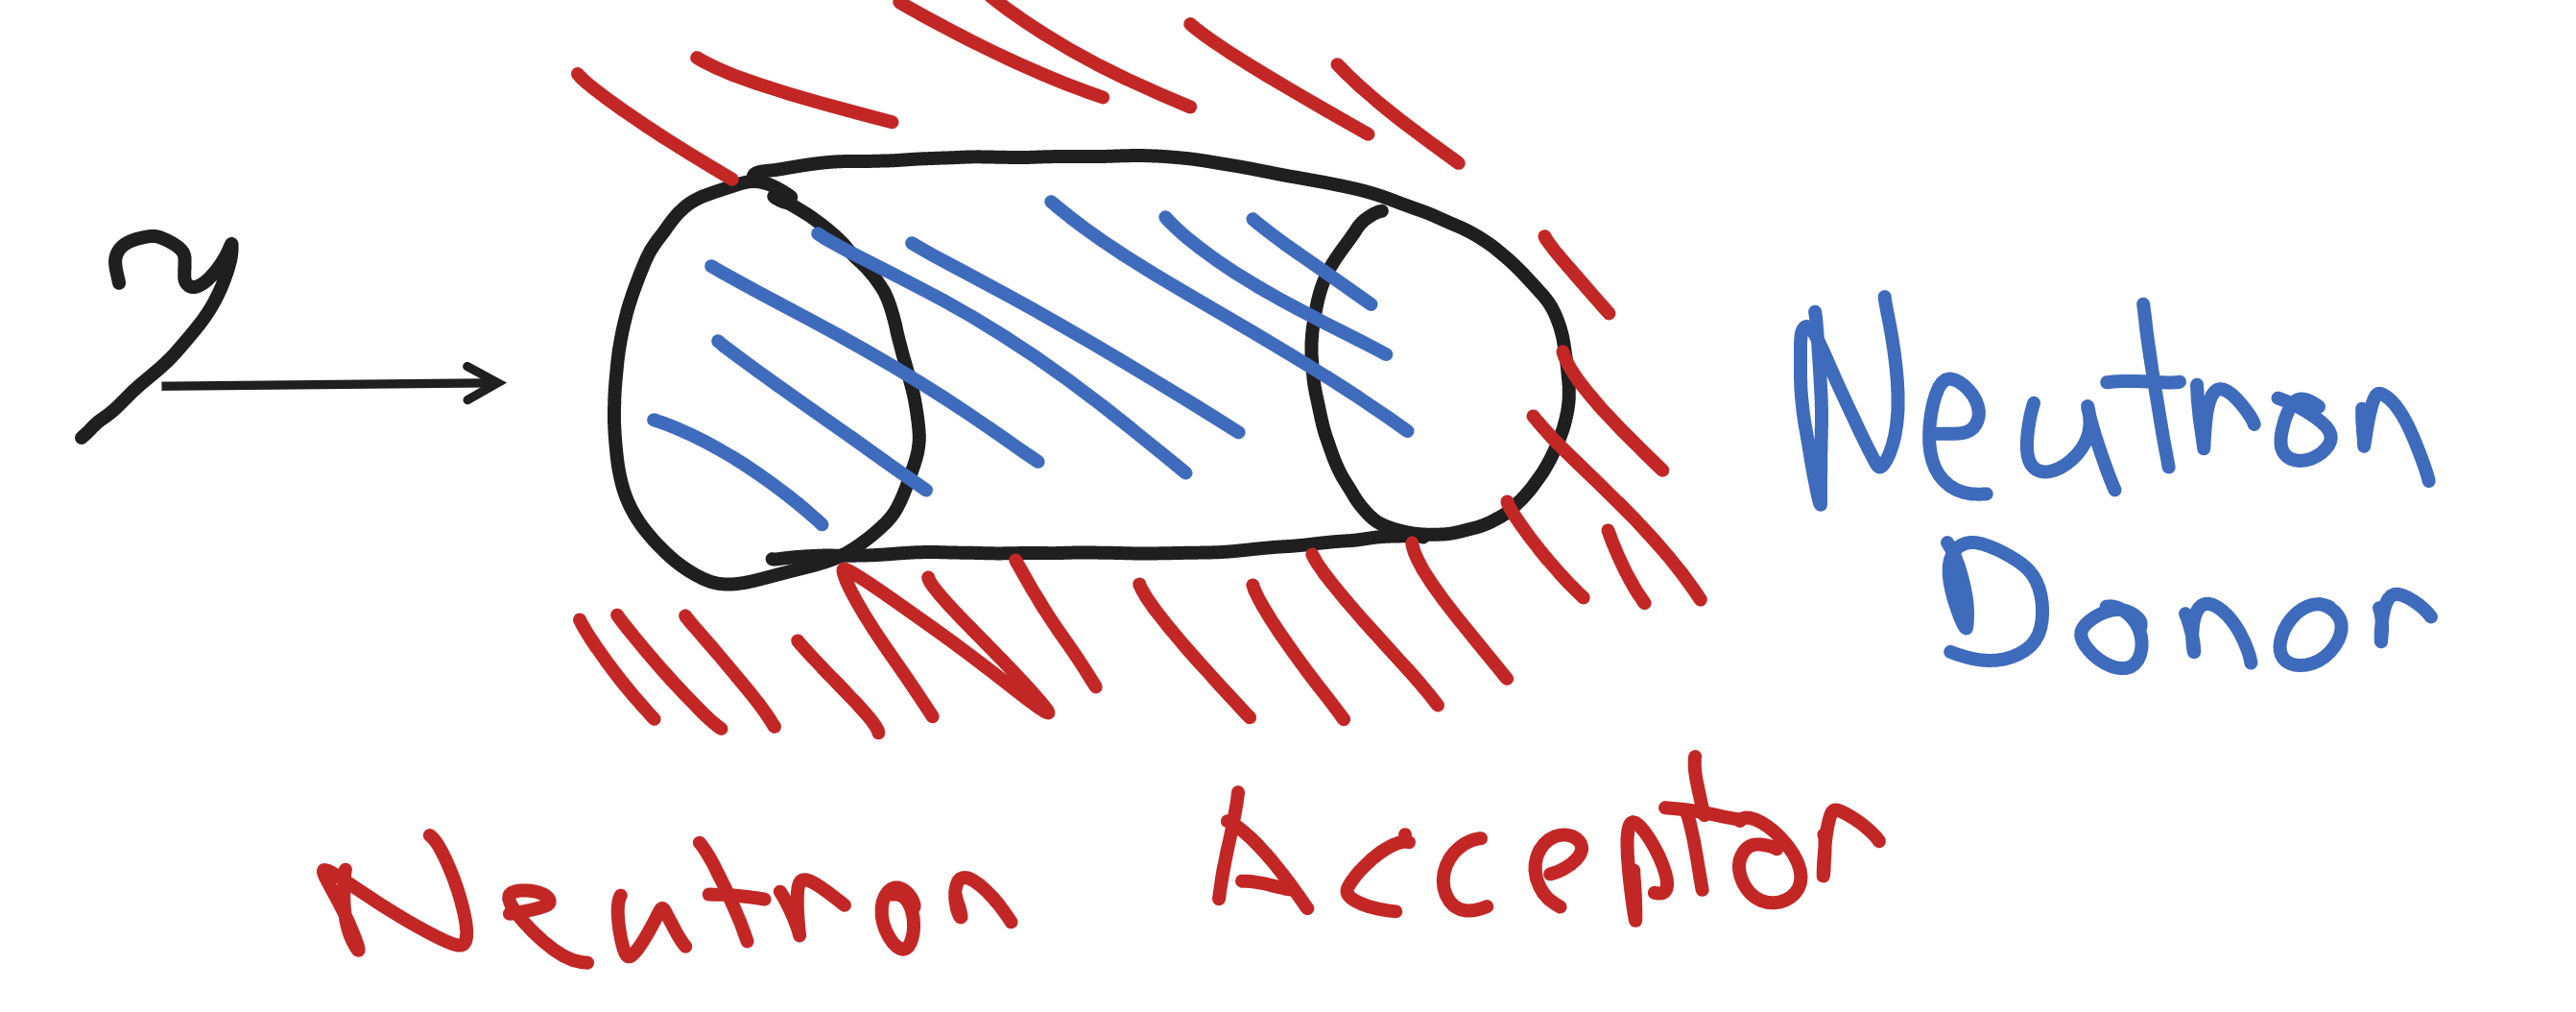
\includegraphics[scale=.4]{Images/concept setup.PNG}\\
In this setup, a gamma ray will be fired at a neutron donor (blue cylinder) which would then be captured by the neutron acceptor (red surroundings). Ideally, the neutron donor would have a very small radius but be a very long cylinder. Assuming every gamma ray produces a neutron which is then capture by the neutron acceptor, it would only cost 1MeV/neutron with deuterium as a neutron donor (leading an energy storage efficiency of $~\frac{1}{3}$ based on the power density of decay chains work since one traverse along each chain yields $300$ keV). Can it's low cross section and density be overcome with this design? What is the ideal neutron acceptor for each neutron donor? Is this less efficient than firing protons into the neutron acceptor? 

\end{document}
